\chapter{Background}

\fixme{TODO: what's in this chapter?}

\section{3D reconstruction}

\fixme{TODO: overview: what is 3D reconstrucion?}

\citet{fabio2003point} overviews the process of converting a point cloud to a 3D polygon mesh and the problems involved. The main contributions of the paper are defining terminology, classifying algorithms and describing the state-of-the-art methods in 2003. No original research is described. Still, the article is helpful in obtaining a very general idea of the process of 3D reconstruction from point cloud data.


\subsection{Point cloud alignment} \label{literature.alignment}

\fixme{TODO: overview: what is this?}
% TODO: mention rigid and non-rigid registration

The Iterative Closest Point (ICP) algorithm is commonly used for aligning two point clouds. The algorithm was originally presented by \citet{besl1992method} and \citet{chen1991object}. A pseudocode description of ICP is shown in algorithm~\ref{literature.pseudoicp}. It works by finding corresponding points from the two point clouds. Then a rigid transformation that minimizes the error between the corresponding point pairs is searched for. This transformation is then applied. Iterating this multiple times, a local optimum should be found.

\begin{algorithm}
\caption{Iterative Closest Point}
\label{literature.pseudoicp}
\begin{algorithmic}
    \For{1..iterations}
        \ForAll{point $x_i$ in X}
            \State $y_i$ = closest point in Y
        \EndFor
        \State error := $sum_i (x_i-y_i)^2$
        \State find rigid transformation $T_i$ that minimizes error
        \State apply $T_i$ on X
    \EndFor
    \State \Return output T = $product_i T_i$
\end{algorithmic}
\end{algorithm}

Even from this description it's obvious that ICP has its shortcomings. If the initial guess is too much off, the algorithm can yield bad results. This is because for non-trivial point clouds, local optima may exist that are significantly different from the global optimum.

Another issue with ICP is that it requires a lot of computation if the point clouds are large. \citet{rusinkiewicz2001efficient} review different ways of improving the efficiency of ICP. They also attain minor improvements to the alignment accuracy.

However, even these improved variants of ICP suffer from converging on local minima. The EM-ICP\footnote{EM in EM-ICP stands for Expectation Maximization (EM), which the algorithm is based on. EM-ICP yields the same results as ICP in the limited circumstances where ICP works well---therefore ICP is included in the name, although the algorithm is fundamentally different.} algorithm introduced by \citet{granger2006multi} overcomes this problem at the cost of being computationally very intensive \citep{tamaki2010softassign}.

\citet{tamaki2010softassign} make EM-ICP more efficient by implementing the computation on GPU using CUDA. The speed is unfortunately still not fast enough for real-time usage on current hardware.

Another interesting improvement over ICP is suggested by \citet{tykkala2011direct}. Their algorithm, Direct Iterative Closest Point, is very well suited for Simultaneous Localization and Mapping (SLAM) using an RGB-D sensor. Direct ICP stores all data in 2D images, thus avoiding expensive 3D nearest neighbor searches. This makes it computationally much cheaper than traditional ICP. The change in approach from 3D point coordinate matching to computing transformations between 2D images also enables using RGB as well as depth data for computation. Using both simultaneously can make the algorithm more robust and accurate. This is demonstrated for deriving the trajectory and pose of a moving camera in static scenery. The downside is that a balancing factor $\lambda$ needs to be chosen. $\lambda$ sets the relative weight between visual and depth components in the minimized cost function.

% TODO: \citep{chui2003new} TPS-RPM \citep{yang2011thin}

\newtopic

The algorithm developed by \citet{huang2011visual} is not point cloud alignment as such, but as it is used to replace ICP in some cases \citep{Whelan12rssw}, it deserves a mention. The article leaves the method unnamed, but an implementation called FOVIS \citep{fovis} is made freely available by the authors. \citet{huang2011visual} aim to create a robust system for stabilizing and controlling an autonomous micro air vehicle (MAV). Their chosen hardware is a quad-rotor MAV that carries a stripped-down Kinect and a small flight computer comprising a 1.86GHz Intel Core 2 Duo processor and 4GB of RAM (Random Access Memory). For autonomous flight, \citeauthor{huang2011visual} develop a visual odometry algorithm that is capable of tracking camera pose and trajectory in real time on the aforementioned hardware--more specifically, computation takes roughly 25ms per frame. The algorithm is image-based and uses RGB-D input, of which the RGB image is converted to grayscale. To enable feature detection at different scales, a Gaussian pyramid is created--in practice, a series of scaled-down images with Gaussian blur. The FAST (Features from Accelerated Segment Test) feature detector \citep{rosten2006machine} is used to extract features at each scale level. Features are matched between frames by computing sum of absolute differences of their feature descriptors, choosing the minimally different features as matches. An initial rotation estimate is calculated by a simple direct pixel error minimization method presented by \citet{mei2009}, and used to restrict feature matches only to the ones that correspond to the general rotation. The matches are further refined by finding the maximal amount of features that are consistent with each other given their locations (using the depth data), assuming a rigid, static scenery. After the feature matching is complete, the locations of each feature are used to find the new camera pose by minimizing feature reprojection error. This error measure is used to still drop possible outlier features, and the pose optimization is done again. Additionally, keyframes are used to reduce local drift in trajectory. As long as the camera motion between keyframe and current frame can be computed with enough inlier features, this result is also considered. When this is no longer possible, the current frame is set as the new keyframe. \citep{huang2011visual}

\subsection{KinectFusion}

\begin{figure}
    \centering
    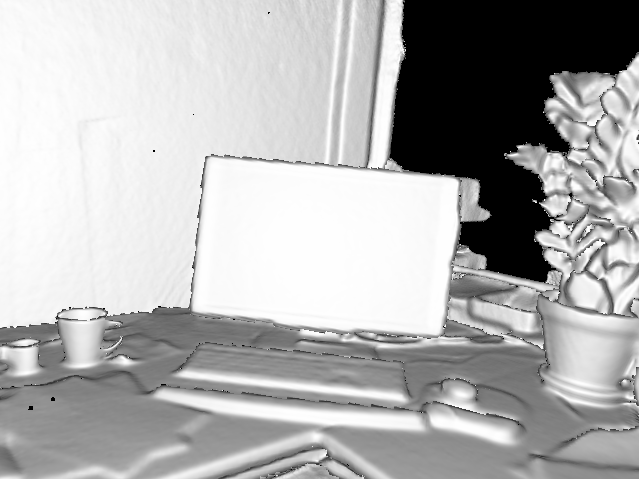
\includegraphics[width=\textwidth]{kinfu-ray.png}
    \caption{Kinfu showing a raytraced view of its TSDF grid, with the camera at the same position as the Kinect is.}
    \label{fig:kinfu-ray}
\end{figure}

\begin{figure}
    \centering
    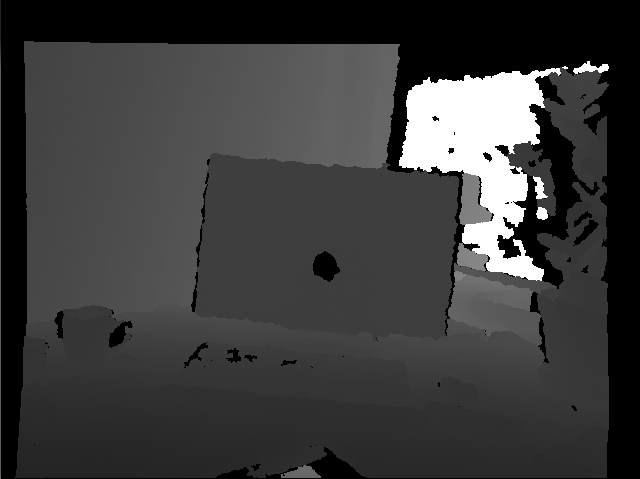
\includegraphics[width=\textwidth]{kinfu-depth.png}
    \caption{The raw depth image from Kinect, at the same moment as the raytraced image in Figure~\ref{fig:kinfu-ray} was drawn.}
    \label{fig:kinfu-depth}
\end{figure}

\begin{figure}
    \centering
    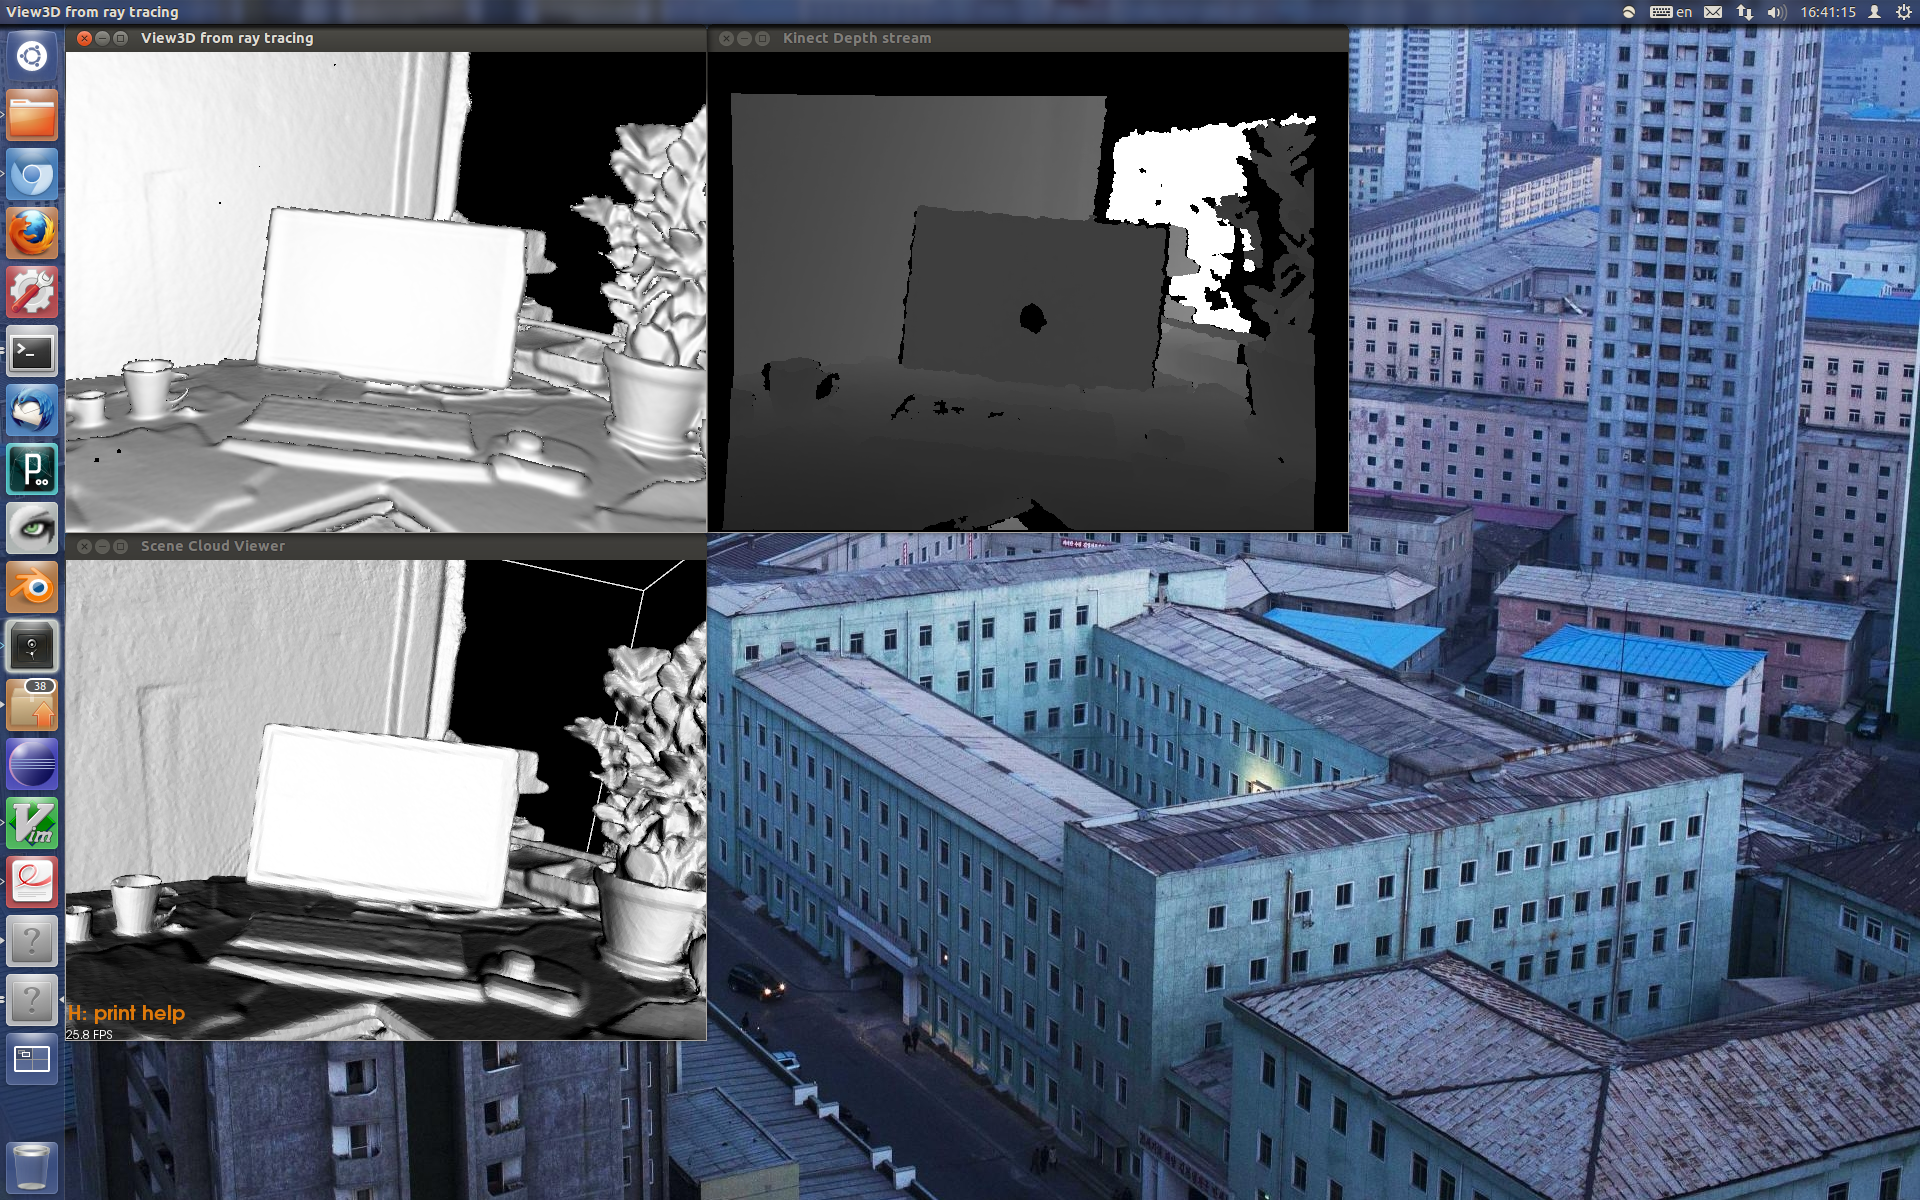
\includegraphics[width=\textwidth]{kinfu-mesh.png}
    \caption{Kinfu showing the mesh generated from the TSDF just moments earlier, with the camera in the same position as in Figure~\ref{fig:kinfu-ray}.}
    \label{fig:kinfu-mesh}
\end{figure}

KinectFusion is a real-time 3D reconstruction system that uses data from a moving Kinect sensor. It performs camera position and pose tracking, surface reconstruction and rendering. \citep{izadi2011kinectfusion}

The implementation works on consumer hardware by way of general-purpose computing on graphics processing units (GPGPU). More specifically, KinectFusion utilizes fully parallel tracking and mapping algorithms that are very efficient on the GPU (graphics processing unit) \citep{newcombe2011kinectfusion}.

KinectFusion uses a variant of Signed Distance Function (SDF), whose value is defined as the distance to the nearest surface for a point in space. The values are signed--a negative value means the point is inside an object. In the KinectFusion implementation, a 3D volume of fixed physical dimensions and resolution is allocated. For each cell in this voxel grid, the distance to nearest surface is saved. Actually, only values for a truncated area near the surface are actually stored--this variation is called Truncated Signed Distance Function (TSDF). \citep{izadi2011kinectfusion}

\fixme{TODO: write a more thorough overview of KinectFusion technology: raycasting, ICP, TSDF/voxel grid}

\newtopic

KinectFusion was made in a project at Microsoft Research and demonstrated using videos, but the software has not been published. Nevertheless, an open source implementation called Kinfu has been made based on the descriptions in the two articles. Kinfu is available as part of the Point Cloud Library (PCL) \citep{PCL}.

The availability of an open source implementation has allowed further improvements on the system. For example, the KinectFusion algorithm was soon improved to work over extended areas \citep{Whelan12rssw}. The enhanced version is called Kintinuous and has been built on Kinfu. Authors of Kintinous have pledged to release the source code back to PCL, but as of writing this has not yet happened. The main contribution of \citet{Whelan12rssw} is to allow moving the TSDF grid, in essence removing the main restriction of KinectFusion that only allows reconstruction of a fixed-size cube (for example, $(3 \mathrm{m})^3$). This is implemented by making the TSDF data structure cyclical--the memory is pre-allocated, but the origin is given by a pointer and can be moved. A threshold is chosen, and when any of the camera coordinates ($x, y, z$) exceeds this threshold, the TSDF is moved. The origin moves to the new camera coordinates. The region no longer in the TSDF is raycasted to find surfaces, which are saved in the main memory. Cells in the TSDF memory that fall outside the new TSDF are marked unmapped, and will be reused to describe a new position. Mesh reconstruction utilizes the algorithm described by \citet{Marton09ICRA}, resulting in a high-polygon surface. The size of the surface is only limited by available memory. \citep{Whelan12rssw}

Another issue pointed out in KinectFusion is that ICP cannot work without geometric features. This shortcoming is alleviated by including FOVIS, the visual odometry algorithm as an alternative to ICP. This is shown to work in real-time, though its CPU implementation is slightly slower than the GPU implementation of ICP. \citep{Whelan12rssw}

Kintinuous was further improved by \citet{Whelan12tr} by adding an image-based tracking algorithm similar to \citep{tykkala2011direct} and the initial step in \citep{huang2011visual}. The three different algorithms used for odometry (ICP, FOVIS and image-based ``RGBD'') can be combined. ICP and RGBD combined can work in real-time and yield a more accurate trajectory than any of the algorithms alone. \citep{Whelan12tr}

Features still lacking in Kintinuous include loop closure and map reintegration. In practice, moving the sensor back to an area already visited is problematic. Since no map reintegration is implemented, the area will be overwritten. Drift may also be significant---no intelligent measures are taken to correct the error when an area is revisited.


\section{Modeling the human body}

\fixme{TODO: overview---animations and games' representation; what are rigged models?}

\fixme{TODO: combine subsections Human body models + 3D reconstruction of the human body}

\subsection{Human anatomy}

Human anatomy is the obvious basis for any artificial model of the human body. Anatomy is not a simple matter; the main anatomical features according to \citetitle{pick1977gray} \citep{pick1977gray} are the skeleton, the articulations, muscles and fasciae, the blood-vascular system, the nervous system and the organs (grouped into six categories). Considering every detail is very impractical--a visually convincing human can be drawn without taking the nervous system into account, for example.

Even though a simplified view of anatomy is enough for visually representing humans, the basics are important. Anatomical knowledge of humans has been employed by visual artists at least since the days of Leonardo da Vinci,
% TODO: Tuukka says sculptors in ancient Greece
who did dissections to gain understanding of the human body \citep{keele1964leonardo}. This was almost three decades before Vesalius, ``the founder of modern human anatomy'' published his seven-volume De humani corporis fabrica \citep{vesalius1543}. \citet{hogarth2003} claims that Titian, the contemporary artist Vesalius asked to produce illustrations, actually knew the visual implications of anatomy better than Vesalius. It is then sensible to consider \term{artistic anatomy} different from \term{medical anatomy}, though they do both exist based on the same truths \citep{hogarth2003}.

To date, several guides to human anatomy for artists have been published \autocites{hogarth2003}{simblet2001}{goldfinger1991}. They vary in depth, but the general requirements for drawing plausible human bodies seem to be an understanding of the skeleton, muscles and skin. Books focusing on just drawing the human form without focus on anatomy still often point this requirement out \autocites{ediciones2004}{loomis1943figure}.

\fixme{TODO: expand this section by writing about one or two sources in more depth}


\subsection{Human body models}

\textit{Morphable models} are defined by \citet{schneider2010fitting} to mean parametric models of 3D shape, created by applying Principal Component Analysis (PCA) on a database of meshes. As a single PCA model can only cover a limited subspace of shapes, complex shapes can be split into parts, creating in essence a multi-PCA model of the overall shape. Fitting such a morphable model to a shape is easy if the target representation is semantically consistent with the model. That is, the target should be a mesh that has the same number of vertices in positions corresponding to the model. Practically, this is rarely true, and a method for finding the correspondences is needed. \citet{schneider2010fitting} describe the classical way of fitting a morphable model to a point cloud that consists of three steps. First, a template mesh corresponding to the vertex structure of the morphable model must be fitted to the point cloud using a non-rigid registration method. This template is used to find points corresponding to vertices. The topology is then solved and the morphable model can be fitted. A better approach is suggested, where all the pose and shape constraints are written as a matrix equation. Then an iterative optimization is run, where the pose is optimized by an ICP-like method, parameter changes are solved from the matrix equation using singular value decomposition and then the parameters are updated. The optimization is stopped when the mean squared error becomes stable between iterations.

A morphable human head model and laser scans of faces are used as an example to show that simultaneous optimization indeed converges faster and produces a more accurate result than using an initial pose optimization and then only fitting shape. Additionally, the 3D head model fitting is shown to work with a mugshot-type set of two 2D images from two directions, by adding more equations to solve for depth. \citep{schneider2010fitting}


The Shape Completion and Animation of People (SCAPE) method developed by \citet{anguelov2005scape} is a data-driven framework for creating a morphable human body model. The model is made low dimensional by decoupling the pose and body shape. The pose model must be learned first by comparing data of the same person in different poses. PCA is used to find deformations for each triangle in the mesh as the function of joint angles. To incorporate body shape variation, the position of each triangle is then defined as the product of pose deformation, body shape deformation and the rotation of the corresponding joint. Given data of different people in arbitrary poses, PCA is used to find a descriptive subspace of body shapes. The model built using these two components is shown to be directly applicable to creating 3D animation. Generating a mesh from parameters took about 1 second when the paper was published in 2005, leading the authors to suggest the method could allow real-time animation in the future. Another demonstrated application is shape completion (for example, from a partial view of a human)--an optimization process for finding pose and shape parameters from incomplete data is derived. Qualitatively, the model seems very capable of approximating the complete 3D human shape from a single incomplete point cloud.

The main limitation of models generated by SCAPE is that the correlation between body shape and muscle deformation cannot be modeled, as the two are decoupled. Practically this means that bodies with a lot of muscular tissue show deformations similar to those with a lot of fatty tissue. Moreover, the deformations are only dependent on joint angles, meaning flexed and relaxed muscles can't be differentiated in the same pose--this also restricts face modeling, as facial expressions are caused by muscular activity, not joint rotations. \citep{anguelov2005scape}

% TODO: \citep{baek2012parametric}


\subsection{3D reconstruction of the human body}

The Master of Research dissertation by \citet{charpentier2011accurate} makes an overview of possible methods at creating avatars with Kinect. Existing methods at creating both sprite-based and 3D avatars are discussed and compared. The working hypothesis is that a Kinect can be used for 3D scanning oneself and making a rigged avatar from the scan. This would allow a much more accurate representation of the user than any of the existing avatar creation tools. Creating a human model is shown to be possible by scanning the person in a static pose from different directions and manually aligning the scans in MeshLab\footnote{MeshLab is an open source application useful for working with point clouds and meshes, available at \url{http://meshlab.sourceforge.net/}} \citep{meshlab}. These aligned scans are then used to create a mesh, which can then be rigged using the Pinocchio software, the prototype implementation of the automatic rigging method introduced by \citep{baran2007automatic}. The result is an animatable avatar that mostly works--however, in the particular case shown one joint is misplaced and there is a long strip of surface between the legs. Texturing is not attempted, and is noted to be slightly problematic due to color differences between the different point clouds. Coloring each vertex using the nearest point color is mentioned as a possible way of texturing the generated mesh. \citep{charpentier2011accurate}

The demonstrated avatar creation method is unwieldy considering that manual alignment takes hours to do. Automatic methods are explored, but no suitable one is found. \citeauthor{charpentier2011accurate} suggests that using KinectFusion to generate the human mesh should make the process easy, if the application was available. \citep{charpentier2011accurate}

\newtopic

Currently, the most promising work at creating personalized human avatars has been by \citet{weiss2011home}. Their approach uses the SCAPE body model \citep{anguelov2005scape}. This makes for very good reconstruction accuracy and excellent representation of the body shape, including realistic deformations in different poses. However, the evaluation is slow at approximately 65 minutes for a human model, according to \citet{weiss2011home} and the SCAPE model needs to be trained with a large amount of data beforehand.
% TODO: expand this

\newtopic

\citet{ahmed2005automatic} presented a method for creating human avatars from multi-view video. The process is automatic and the avatars are visually quite accurate. For capturing, a frame-synchronized setup of eight cameras is used. The human is segmented from each view, yielding eight silhouettes. A template body model is deformed so that it optimally fits all the silhouettes. The template consists of 16 parts, each of which is controlled by four B-splines. The deformations are optimized for each viewpoint, and for improved accuracy, using several non-subsequent frames. According to the authors, about five automatically chosen time steps are sufficient, and thus just a few seconds of multi-view video is required. The computation of the human model takes about 15 minutes. After the shape is personalized, it is textured by projecting the images back to the constructed model. The method takes occlusion into account and combines textures over several time steps. The texture reconstruction takes around 40 seconds. As an additional feature, the user can manually select frames with interesting facial expressions. These expressions can then be changed on the avatar. \citep{ahmed2005automatic}

\newtopic

\citet{stoll2010video} capture animatable virtual humans from multi-view video similar to what \citet{ahmed2005automatic} use, making the reconstruction more accurate and adding cloth modeling, while not implementing texturing. They show algorithms for identifying cloth and estimating its parameters for cloth simulation, and guessing the surface geometry underneath the clothing. The cloth capture and simulation is shown to be plausible by a user study. Computation of the model takes 2.5 hours for 1000 frames of multi-view video, but afterwards the model can be animated in real time using a rigged skeleton. \citep{stoll2010video}

\citet{tongscanning} use three Kinects and a turntable to scan human bodies. Their method requires the human to be standing in a static pose for 30 seconds, while the turntable rotates 360 degrees. The method starts by creating a very simplified template mesh of the human in first frame. This mesh is used to find the changes between each consecutive pair of frames. After the full rotation, the error sum of the pairwise registration can be calculated, and it is spread evenly across all the frames--similar to how loop closure works in SLAM systems. The authors note a better accuracy than \citep{weiss2011home}, which is due to the latter using a human shape model (SCAPE) that is only applicable to near-naked human bodies. In practice, the method by \citeauthor{tongscanning} is capable of modeling arbitrary surfaces on top of the human such as clothes and hair. It can also work with shapes that are not included in the SCAPE space, such as specific facial features not interpolatable from the SCAPE training data. However, this comes at the cost of animation. Whereas SCAPE supports freeform posing and has realistic deformations \citep{anguelov2005scape}, \citet{tongscanning} only note that the ``skeleton and skin weights of the reconstructed body mesh can be automatically extracted'' using another method such as \citep{baran2007automatic}.

\newtopic

The work of \citet{hirshbergc2011evaluating} focuses on aligning human laser scans from different directions. They develop methods for automatically locating the two ankles and the sellion landmark, defined as ``Point of greatest indentation of the nasal root depression'' \citep{blackwell2002civilian}. These three points are shown to be enough for accurate scan alignment of data in the CAESAR dataset \citep{robinette2002civilian}. The article makes no mention of problems with viewpoints where the face is mostly occluded, but the sellion detection method is based on face detection. This seems like a major oversight.
% TODO: go deeper

% TODO: (human pose) \citep{baak2011data} \citep{pekelny2008articulated} \citep{droeschel20113d}


\subsection{MakeHuman} \label{literature.makehuman}

MakeHuman \citep{makehuman} is an open source software application for 3D human modeling.

MakeHuman has an androgynous base mesh that supposedly depicts an average human. It can be modified in diverse ways using a number of predefined \term{targets} that define deformations. A commendable amount of work has been put into refining the base mesh and targets. Initially it seems like an arbitrary human could be accurately modeled using MakeHuman, given enough time for fine-tuning.

\begin{figure}
    \centering
    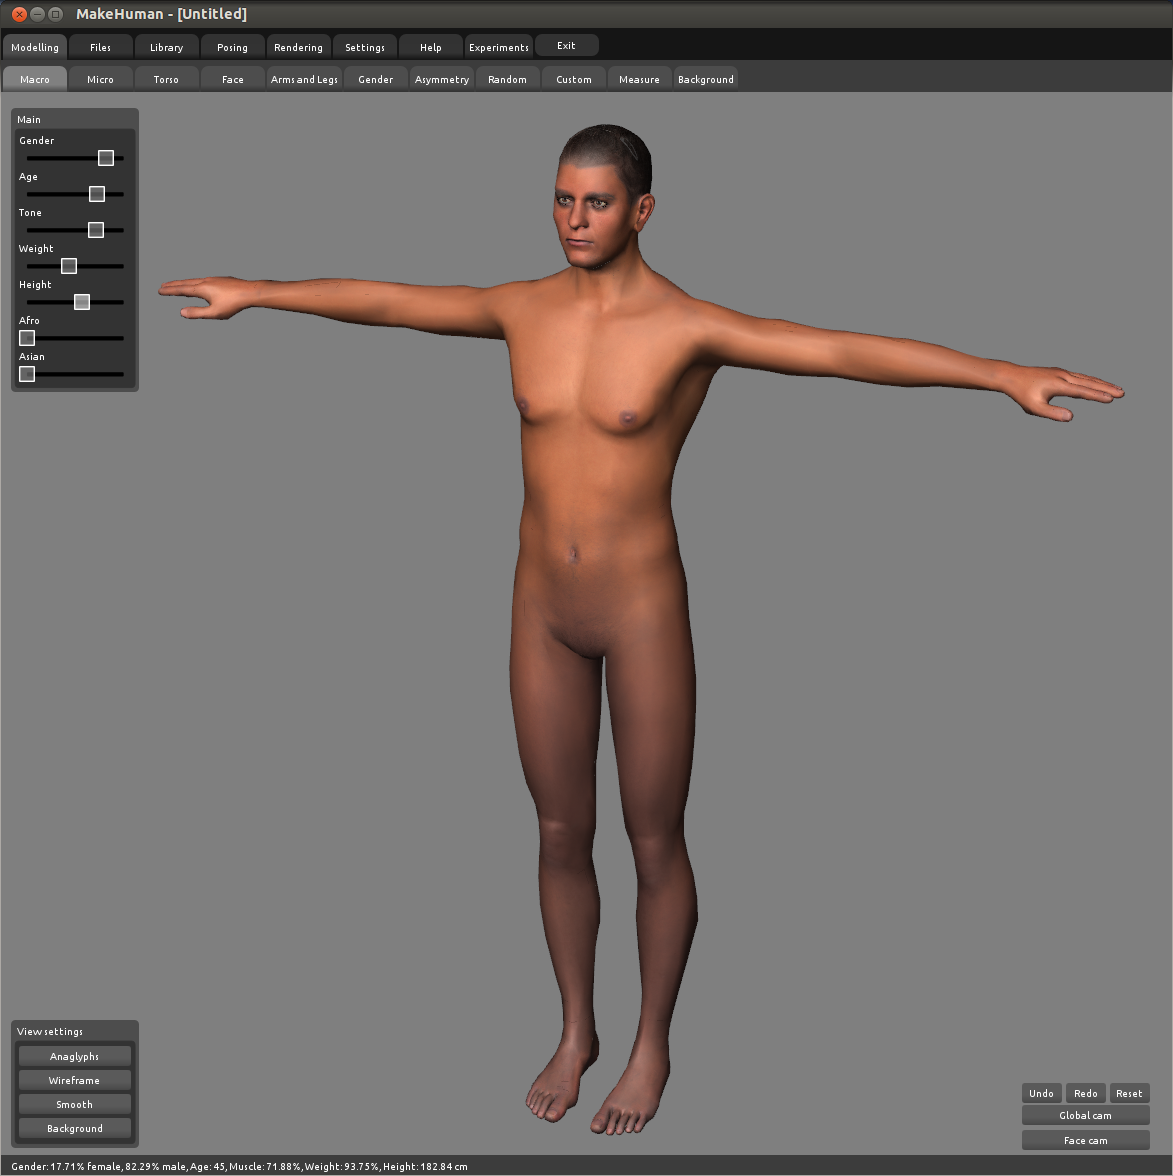
\includegraphics[width=\textwidth]{makehuman-male.png}
    \caption{MakeHuman showing a middle-aged male and the macro controls.}
    \label{fig:makehuman-male}
\end{figure}

\begin{figure}
    \centering
    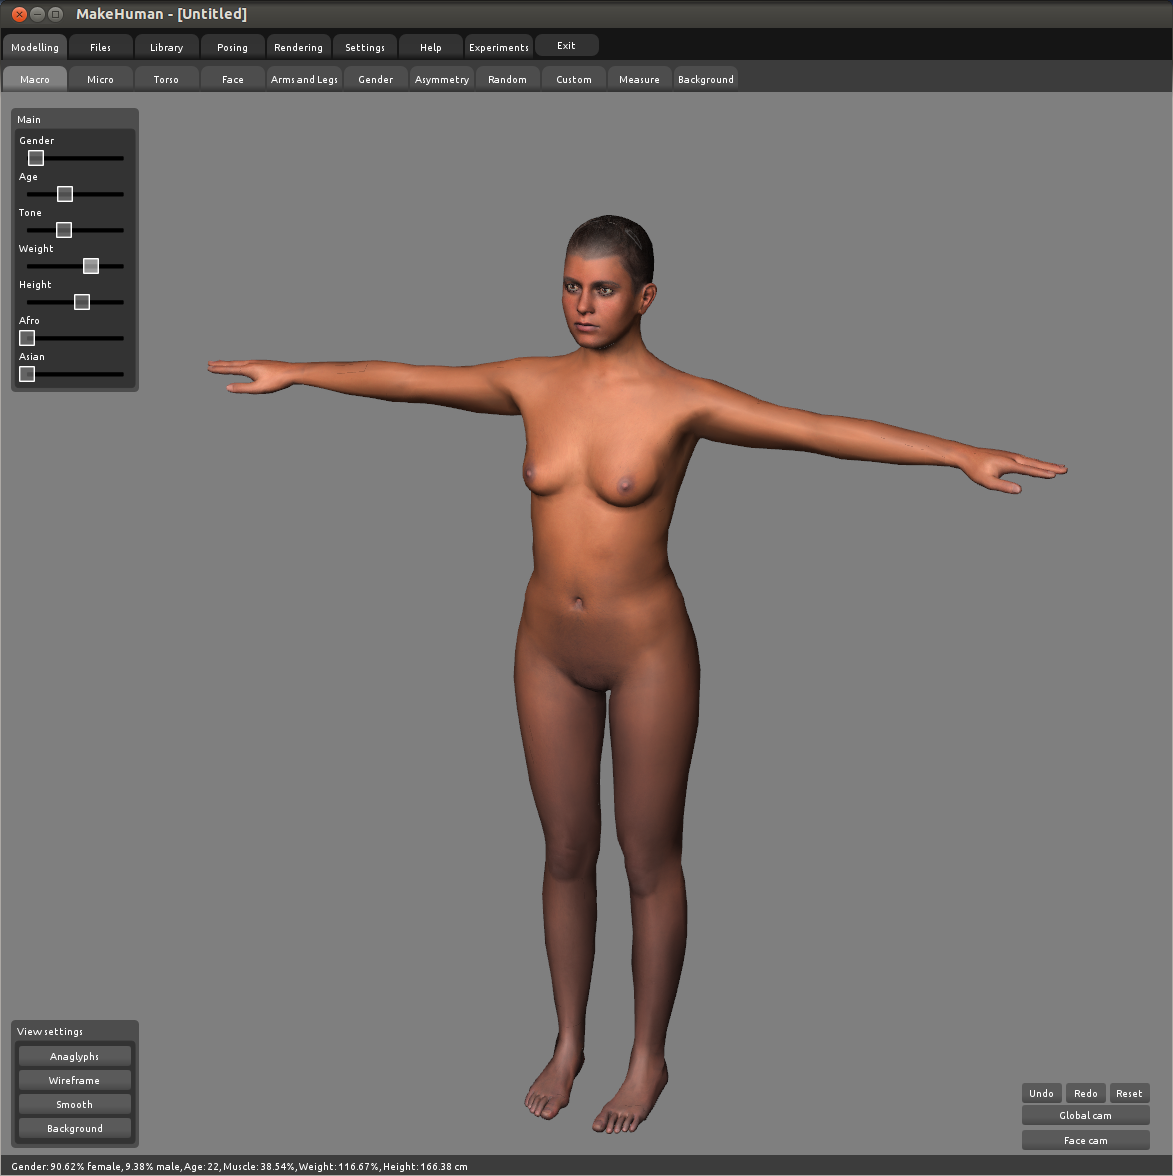
\includegraphics[width=\textwidth]{makehuman-female.png}
    \caption{A young female modeled using MakeHuman.}
    \label{fig:makehuman-female}
\end{figure}

Modeling different kinds of people is very easy using the MakeHuman application. For example, both the middle-aged male in figure \ref{fig:makehuman-male} and the young female in \ref{fig:makehuman-female} are made in MakeHuman by changing a couple of the major parameters. Getting from one to the other only takes a few drags of sliders and a couple of seconds. Of course, more detailed changes are possible and tuning them by hand might take time. To give a general idea of the broadness, there are over a hundred targets in 15 categories just for facial features.

Technically, the base mesh used by MakeHuman has indexed vertices, each with its own coordinates. Each target defines a vector for each vertex---this is often zero for most vertices, in which case only the non-zero vectors are actually stored. A target can be applied with a weight that is a real number, usually chosen between 0.0 and 1.0. Zero is the default, meaning the target does not change the mesh. When targets weights are changed, the coordinates for each vertex are recalculated as
%
\begin{equation*}
    \vec{v}_i = \vec{b}_i + w_1 \vec{t}_{1,i} + w_2 \vec{t}_{2,i} + \dots  + w_n \vec{t}_{n,i},
\end{equation*}
%
where $i$ is the index of the vertex, $\vec{v}_i$ are the calculated coordinates of the vertex, $\vec{b}_i$ are the coordinates of the vertex in the base mesh, $w_k$ is the weight applied to the $k$th target and $\vec{t}_{k,i}$ is the vector defined for the $i$th vertex in the $k$th target.

Using this system, the order of the targets does not matter. The mesh need not be recalculated from the beginningon each change, either---only the difference caused by changed targets must be calculated and added to the current coordinates.


\section{Sensor driver software} \label{literature.drivers}

When the work on this thesis began, at least three different drivers for Kinect were available. 

\subsection{Microsoft Kinect SDK}

The obvious solution for developing software that uses Kinect is the Microsoft Kinect for Windows Software Development Kit (SDK) \citep{KinectSDK}. While Kinect is a Microsoft product, Microsoft actually only released the SDK after open-source drivers had gained momentum. Therefore, while Microsoft SDK strives to be the standard, the de facto standard actually still seems to be OpenNI instead.

The Microsoft SDK is available for Windows 7 and later. It supports development in C++/CLI, C\# or Visual Basic .NET. A multitude of features have been included in the SDK. For example, skeleton tracking, face tracking and audio input are supported.

License restrictions in the Microsoft Kinect SDK make it unappealing. For example, using a Microsoft Kinect for Xbox 360 is allowed for development, but distributing Microsoft SDK--based software for use with it is forbidden. Only using a Microsoft Kinect for Windows sensor is allowed for end-users. This is required to be ``clearly stated'' in all materials related to any created application. Moreover, the end-user license agreement (EULA) forbids applying a copyleft license to applications created using the Microsoft SDK. \citep{kinectEULA}

\subsection{OpenKinect}

OpenKinect \citep{openkinect} is an open community project aiming at creating open-source software for using Kinect. The focus of the project is the libfreenect library, available under the terms of Apache License 2.0 \citep{Apache2} or the GNU General Public License (GPL) 2.0 \citep{GPL2}.

OpenKinect is made from scratch by hobbyists, and remains very low-level. It is possible to read video and depth data, but combining them to create point clouds is not supported by libfreenect. \citet{burrus2010} shows a workable calibration procedure, and also shares the measured calibration parameters for others to use. \citet{fisher2010} shows example code of using these parameters to transform video and depth images to colored points in world coordinates.

Tilting the Kinect using the built-in motor and changing the color of the led are also supported by libfreenect. While not particularly useful in most applications, these features are notable as they are missing from OpenNI, the other freely available driver.

\subsection{OpenNI}

The OpenNI (Open Natural Interaction) library \citep{OpenNI} is developed by PrimeSense, which also manufactures the sensor hardware used in Microsoft Kinect and the Asus Xtion series. OpenNI is available under the GNU Lesser General Public License (LGPL), version 3 \citep{LGPL3}. Packages of OpenNI are provided for Windows, Ubuntu and Mac OS X.

OpenNI supports embedding middleware that can greatly enhance functionality of the library. PrimeSense leverage this architecture by supplying a proprietary middleware called NITE (Natural Interaction Technology for End-user) \citep{NITE}. Binary packages of NITE are available for Windows, Ubuntu and Mac OS X on the download section of the OpenNI website \citep{OpenNI}. No license terms are mentioned on the download page nor during the installation. In the past, NITE came with an EULA restricting it to only be used with sensors manufactured by PrimeSense. While the licensing is slightly unclear, the openness of OpenNI leaves hope for an open source middleware replacing NITE.

OpenNI has support for different kinds of input from sensors, including audio, video, depth image and point clouds. NITE includes more advanced features such as user segmentation and skeleton reconstruction.

